\section{A Technique for Debugging A Distributed R-Tree}
\label{sec:rdebug}

Guarantee that a distributed spatial index has being built accordingly is a non-trivial task. 
In a distributed environment, it is hard to find bugs on insertion algorithms due the difficult to synchronize the insertion, since it must be done concurrently.
Even in cases where the implementation is correct, it is not easy to improve the insertion algorithm's performance (for example reducing the overlapping) 
due the intricacy to collect information about the spatial index.

This section describes RDebug, a new technique for index debugging, which allows collect debugging information about the distributed spatial index once it has been created. 
The following debug information about building consistency of the R-Tree index are collected by RDebug: 
i) if each R-Tree node N are consistent between the servers that store any replica of N;
ii) if the MBR of each parent node intersects with the MBR of their children, 
iii) the presence of duplicated nodes on R-Tree or nodes being referenced by more than one parent node, and 
iv) if the value M and m of the nodes are compliant with the R-Tree descriptions as shown in Section \ref{sec:spatial_dist}. 
Furthermore, it is possible to access index data to help in optimization and minimizing  the dead space and overlapping area.

The RDebug algorithm was based on R-Tree structure because it is used to index the spatial datasets on DistGeo platform presented in our work on Sub-Section \ref{sub:dist_geo}.
RDebug can be used with any index similar to R-Tree like Hilbert R-Tree \cite{kamel1994hilbert}, 
since the RDebug algorithm uses the nodes organization of the R-Tree to collect the debug information.

Algorithm \ref{alg:rdebug} shows the RDebug technique for debugging the distributed spatial index, using the index structure itself. The algorithm has two steps:
1) The algorithm processing is similar to the search in an R-Tree with a top-down traversal; 
2) The algorithm does a bottom-up traversal on R-Tree, constructing the result with the debug information.

RDebug has been implemented on DistGeo platform. The R-Tree nodes are distributed and replicated over the cluster. 
Thus, RDebug can be processed on DistGeo platform without bottlenecks and point of failures. 
Besides, the R-Tree replicated nodes in the cluster allow load-balancing in the distributed R-Tree index traversal. 
During the traversal, at every node accessed the traversal might go to a node of the cluster with less workload, increasing the RDebug algorithm performance. 

\medskip
\begin{center}
\begin{minipage}{1\textwidth}
\begin{algorithm2e}[H]
\SetAlFnt{\small\sf}
 \DontPrintSemicolon
 \LinesNumbered
\SetAlgoLined
 \BlankLine
 \KwData{$T$ reference of the root node of R-Tree $tree$}
 \KwResult{Debugging information about distributed R-Tree $tree$}
 \BlankLine

 S1 [Search subtrees]

\eIf{$T$ is not leaf}{
  stores the number of children entries in each replica server of T\;
  \For{each entry $E$ in $T$} {
       $server \leftarrow $ choose one server, randomly,  that keep one replica of $E$\;
           send msg to $server$ to process the node's child of $E$ on step S1\;
   }
}
{
  verify the consistency of $T$ in other replicas\;
      Invoke step S2 [Aggregation]\;
}

S2 [Aggregation]

$information \Leftarrow$ the child's information stored on shared memory by replicas of $T$\;
$replica\_consistency \Leftarrow$ verify the consistency of $T$ in others replicas\;
$node\_consistency \Leftarrow$	verify the consistency of $M$ and $m$ values of  $T$\;
$overlap \Leftarrow$ overlap area of $T$\;
$dead\_area \Leftarrow$ dead area of $T$\;
$bound \Leftarrow$ MBR of $T$\;
add in $information$: $replica\_consistency$, $node\_consistency$, $overlap$, $dead\_area$, $bound$\;

\eIf{$T$ is leaf}{
 \If{$T$ is root}{
       send response with R-Tree nodes information to app client\;
   }
{
    send msg with $information$ to parent of $T$\;
}
}
{
$entry\_info \Leftarrow$ information sent by child node\;
$mbr\_consistent \Leftarrow$ verify if the bound of the child node is equal to bound of entry of T that points to this child\;
add in $information$: $entries\_info$, and $mbr\_consistent$\;
$count \Leftarrow$ retrieve the number of child entries, which did not send a debugging response and decrement by 1\;

 \eIf{$count$ == 0}{
    \eIf{$T$ is root}{
       send response with $information$ to client\;
     }
{
 send msg with $information$ to parent of $T$\;
}    
}
{
store $information$ on shared memory\;
}
          
}
\caption{$RDebug(T)$ 
\label {alg:rdebug}}
\end{algorithm2e}
\end{minipage}
\end{center}

In the first step, called S1 [Search sub-trees] (lines 1 - 11), the Algorithm \ref{alg:rdebug} traverses every node of the R-Tree starting from the root node to the leaves.
The first request is sent to any server, which stores a replica of the root node.

If the node $T$ is not a leaf (lines 2 - 8), then the number of children entries is stored to control the number of expected answers associated to $T$ in the second step of the algorithm. 
This information is stored in a shared memory accessed by all servers with a replica of $T$. Lines $4-7$, show that for each entry $E$ in $T$, 
a message is sent (continuing step S1) to any server that holds a replica of the child node of $E$, carrying on the first step in the children nodes. 
If $T$ is a leaf, the second step, named S2 [Aggregation] is started.

Second step aims (lines $12-39$) to aggregate the information about the index to be used for future debugging.
This step returns debugging information about each node of the R-Tree.
The index itself is used to aggregate this information using the cluster computational resources to improve the algorithm's performance.
The index reverse structure facilitates the collection of the debugging information, 
as one node of the R-Tree is responsible to aggregate only the information of its children. 

The debug information about each node of R-Tree in stored in a shared memory that can be accessed by any server that store a replica of $T$.
The RDebug update the information about the node $T$ that is being analyzed between the lines $13-18$.

In the line 13, the information is retrieved from the shared memory. 
Line 14 verifies the consistency of $T$ in the servers that store any replica of $T$. Line 15 verifies the consistency of $M$ and $m$ values. 
Lines 16 and 17 calculate the overlap and the dead space area, respectively, for each node of the R-tree. 
Line 18 get the MBR of the $T$. This information is inserted in $information$ on line 18.

If the aggregation step is being executed in the leaves (lines 20 - 24), then there are two options.
If $T$ is the root node (line 22), the node information is sent to the client application. 
If $T$ is not the root node, in line 24, the information is sent to the parent node of $T$. 

If the aggregation step is in an internal node (lines 26 - 39), the algorithm aggregates the information of the children nodes. 
In the line 29, the algorithm receives the information sent by the child node. 
Line 27, verifies if the MBR of the entry that points to the child node is indeed the same MBR sent by the child node.
	
Line 28 adds the data processed from lines 26 and 27 in $information$. Line 29 acquires the number of children nodes that not sent debugging information yet. 
This value is stored in the variable $count$, which is decremented and updated on shared memory.
	
If every node has sent the answer, the variable count then will hold the value 0 and lines 30-35 are processed. 
If $T$ is the root node, then the information is sent to the client application, otherwise, all information collected is sent to the parent node of $T$. 
If the variable $count$ is greater than 0, then the client information is stored in the shared memory to be used until until each reply is received by child nodes.
	
The algorithm \ref{alg:rdebug} was implemented in the DistGeo platform to collect the debugging information of the built distributed R-tree. 
This information is used in the platform to find out indexing issues and for speed up the searching on an R-Tree.
Using RDebug algorithm it is possible debug the searching algorithms in a single R-Tree. 
For example, the Window Query algorithm shown on Section \ref{sec:spatial_dist}. 
Whereas, algorithms that access many R-Trees, such as Spatial Join, need a deep change, as the algorithms can go through different paths.

\begin{figure}[ht]
  \centering
  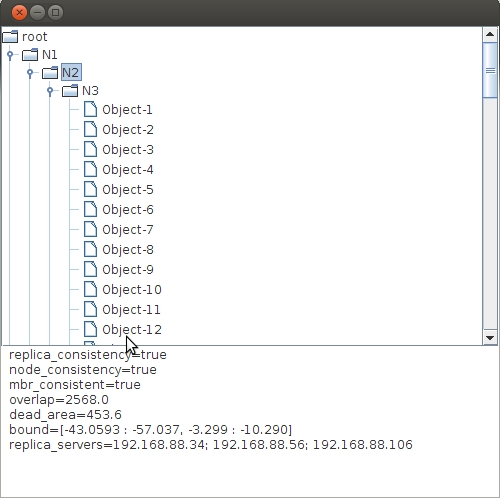
\includegraphics[width=0.5\textwidth]{rdebug-vis.jpg}
  \caption{RDebug Visualizer}
  \label{fig:rdebug-vis}
\end{figure}

The algorithm RDebug have collected debugging information about the R-Tree index built during the insertion of the dataset.
Figure \ref{fig:rdebug-vis} shows a graphical tool (RDebug Visualizer) created in our work to visualize the collected debugging information.
RDebug Visualizer shows the structure of the distributed R-Tree index and allows the analysis of each node of the R-Tree.
The output of the RDebug algorithm shows which nodes are currently inconsistent.
The user can access the path of the node and visualize the node's inconsistent information.    